
\documentclass[10pt]{article} % For LaTeX2e
\usepackage[preprint]{tmlr}
% If accepted, instead use the following line for the camera-ready submission:
%\usepackage[accepted]{tmlr}
% To de-anonymize and remove mentions to TMLR (for example for posting to preprint servers), instead use the following:
%\usepackage[preprint]{tmlr}

% Optional math commands from https://github.com/goodfeli/dlbook_notation.
%%%%% NEW MATH DEFINITIONS %%%%%

\usepackage{amsmath,amsfonts,bm}

% Mark sections of captions for referring to divisions of figures
\newcommand{\figleft}{{\em (Left)}}
\newcommand{\figcenter}{{\em (Center)}}
\newcommand{\figright}{{\em (Right)}}
\newcommand{\figtop}{{\em (Top)}}
\newcommand{\figbottom}{{\em (Bottom)}}
\newcommand{\captiona}{{\em (a)}}
\newcommand{\captionb}{{\em (b)}}
\newcommand{\captionc}{{\em (c)}}
\newcommand{\captiond}{{\em (d)}}

% Highlight a newly defined term
\newcommand{\newterm}[1]{{\bf #1}}


% Figure reference, lower-case.
\def\figref#1{figure~\ref{#1}}
% Figure reference, capital. For start of sentence
\def\Figref#1{Figure~\ref{#1}}
\def\twofigref#1#2{figures \ref{#1} and \ref{#2}}
\def\quadfigref#1#2#3#4{figures \ref{#1}, \ref{#2}, \ref{#3} and \ref{#4}}
% Section reference, lower-case.
\def\secref#1{section~\ref{#1}}
% Section reference, capital.
\def\Secref#1{Section~\ref{#1}}
% Reference to two sections.
\def\twosecrefs#1#2{sections \ref{#1} and \ref{#2}}
% Reference to three sections.
\def\secrefs#1#2#3{sections \ref{#1}, \ref{#2} and \ref{#3}}
% Reference to an equation, lower-case.
\def\eqref#1{equation~\ref{#1}}
% Reference to an equation, upper case
\def\Eqref#1{Equation~\ref{#1}}
% A raw reference to an equation---avoid using if possible
\def\plaineqref#1{\ref{#1}}
% Reference to a chapter, lower-case.
\def\chapref#1{chapter~\ref{#1}}
% Reference to an equation, upper case.
\def\Chapref#1{Chapter~\ref{#1}}
% Reference to a range of chapters
\def\rangechapref#1#2{chapters\ref{#1}--\ref{#2}}
% Reference to an algorithm, lower-case.
\def\algref#1{algorithm~\ref{#1}}
% Reference to an algorithm, upper case.
\def\Algref#1{Algorithm~\ref{#1}}
\def\twoalgref#1#2{algorithms \ref{#1} and \ref{#2}}
\def\Twoalgref#1#2{Algorithms \ref{#1} and \ref{#2}}
% Reference to a part, lower case
\def\partref#1{part~\ref{#1}}
% Reference to a part, upper case
\def\Partref#1{Part~\ref{#1}}
\def\twopartref#1#2{parts \ref{#1} and \ref{#2}}

\def\ceil#1{\lceil #1 \rceil}
\def\floor#1{\lfloor #1 \rfloor}
\def\1{\bm{1}}
\newcommand{\train}{\mathcal{D}}
\newcommand{\valid}{\mathcal{D_{\mathrm{valid}}}}
\newcommand{\test}{\mathcal{D_{\mathrm{test}}}}

\def\eps{{\epsilon}}


% Random variables
\def\reta{{\textnormal{$\eta$}}}
\def\ra{{\textnormal{a}}}
\def\rb{{\textnormal{b}}}
\def\rc{{\textnormal{c}}}
\def\rd{{\textnormal{d}}}
\def\re{{\textnormal{e}}}
\def\rf{{\textnormal{f}}}
\def\rg{{\textnormal{g}}}
\def\rh{{\textnormal{h}}}
\def\ri{{\textnormal{i}}}
\def\rj{{\textnormal{j}}}
\def\rk{{\textnormal{k}}}
\def\rl{{\textnormal{l}}}
% rm is already a command, just don't name any random variables m
\def\rn{{\textnormal{n}}}
\def\ro{{\textnormal{o}}}
\def\rp{{\textnormal{p}}}
\def\rq{{\textnormal{q}}}
\def\rr{{\textnormal{r}}}
\def\rs{{\textnormal{s}}}
\def\rt{{\textnormal{t}}}
\def\ru{{\textnormal{u}}}
\def\rv{{\textnormal{v}}}
\def\rw{{\textnormal{w}}}
\def\rx{{\textnormal{x}}}
\def\ry{{\textnormal{y}}}
\def\rz{{\textnormal{z}}}

% Random vectors
\def\rvepsilon{{\mathbf{\epsilon}}}
\def\rvtheta{{\mathbf{\theta}}}
\def\rva{{\mathbf{a}}}
\def\rvb{{\mathbf{b}}}
\def\rvc{{\mathbf{c}}}
\def\rvd{{\mathbf{d}}}
\def\rve{{\mathbf{e}}}
\def\rvf{{\mathbf{f}}}
\def\rvg{{\mathbf{g}}}
\def\rvh{{\mathbf{h}}}
\def\rvu{{\mathbf{i}}}
\def\rvj{{\mathbf{j}}}
\def\rvk{{\mathbf{k}}}
\def\rvl{{\mathbf{l}}}
\def\rvm{{\mathbf{m}}}
\def\rvn{{\mathbf{n}}}
\def\rvo{{\mathbf{o}}}
\def\rvp{{\mathbf{p}}}
\def\rvq{{\mathbf{q}}}
\def\rvr{{\mathbf{r}}}
\def\rvs{{\mathbf{s}}}
\def\rvt{{\mathbf{t}}}
\def\rvu{{\mathbf{u}}}
\def\rvv{{\mathbf{v}}}
\def\rvw{{\mathbf{w}}}
\def\rvx{{\mathbf{x}}}
\def\rvy{{\mathbf{y}}}
\def\rvz{{\mathbf{z}}}

% Elements of random vectors
\def\erva{{\textnormal{a}}}
\def\ervb{{\textnormal{b}}}
\def\ervc{{\textnormal{c}}}
\def\ervd{{\textnormal{d}}}
\def\erve{{\textnormal{e}}}
\def\ervf{{\textnormal{f}}}
\def\ervg{{\textnormal{g}}}
\def\ervh{{\textnormal{h}}}
\def\ervi{{\textnormal{i}}}
\def\ervj{{\textnormal{j}}}
\def\ervk{{\textnormal{k}}}
\def\ervl{{\textnormal{l}}}
\def\ervm{{\textnormal{m}}}
\def\ervn{{\textnormal{n}}}
\def\ervo{{\textnormal{o}}}
\def\ervp{{\textnormal{p}}}
\def\ervq{{\textnormal{q}}}
\def\ervr{{\textnormal{r}}}
\def\ervs{{\textnormal{s}}}
\def\ervt{{\textnormal{t}}}
\def\ervu{{\textnormal{u}}}
\def\ervv{{\textnormal{v}}}
\def\ervw{{\textnormal{w}}}
\def\ervx{{\textnormal{x}}}
\def\ervy{{\textnormal{y}}}
\def\ervz{{\textnormal{z}}}

% Random matrices
\def\rmA{{\mathbf{A}}}
\def\rmB{{\mathbf{B}}}
\def\rmC{{\mathbf{C}}}
\def\rmD{{\mathbf{D}}}
\def\rmE{{\mathbf{E}}}
\def\rmF{{\mathbf{F}}}
\def\rmG{{\mathbf{G}}}
\def\rmH{{\mathbf{H}}}
\def\rmI{{\mathbf{I}}}
\def\rmJ{{\mathbf{J}}}
\def\rmK{{\mathbf{K}}}
\def\rmL{{\mathbf{L}}}
\def\rmM{{\mathbf{M}}}
\def\rmN{{\mathbf{N}}}
\def\rmO{{\mathbf{O}}}
\def\rmP{{\mathbf{P}}}
\def\rmQ{{\mathbf{Q}}}
\def\rmR{{\mathbf{R}}}
\def\rmS{{\mathbf{S}}}
\def\rmT{{\mathbf{T}}}
\def\rmU{{\mathbf{U}}}
\def\rmV{{\mathbf{V}}}
\def\rmW{{\mathbf{W}}}
\def\rmX{{\mathbf{X}}}
\def\rmY{{\mathbf{Y}}}
\def\rmZ{{\mathbf{Z}}}

% Elements of random matrices
\def\ermA{{\textnormal{A}}}
\def\ermB{{\textnormal{B}}}
\def\ermC{{\textnormal{C}}}
\def\ermD{{\textnormal{D}}}
\def\ermE{{\textnormal{E}}}
\def\ermF{{\textnormal{F}}}
\def\ermG{{\textnormal{G}}}
\def\ermH{{\textnormal{H}}}
\def\ermI{{\textnormal{I}}}
\def\ermJ{{\textnormal{J}}}
\def\ermK{{\textnormal{K}}}
\def\ermL{{\textnormal{L}}}
\def\ermM{{\textnormal{M}}}
\def\ermN{{\textnormal{N}}}
\def\ermO{{\textnormal{O}}}
\def\ermP{{\textnormal{P}}}
\def\ermQ{{\textnormal{Q}}}
\def\ermR{{\textnormal{R}}}
\def\ermS{{\textnormal{S}}}
\def\ermT{{\textnormal{T}}}
\def\ermU{{\textnormal{U}}}
\def\ermV{{\textnormal{V}}}
\def\ermW{{\textnormal{W}}}
\def\ermX{{\textnormal{X}}}
\def\ermY{{\textnormal{Y}}}
\def\ermZ{{\textnormal{Z}}}

% Vectors
\def\vzero{{\bm{0}}}
\def\vone{{\bm{1}}}
\def\vmu{{\bm{\mu}}}
\def\vtheta{{\bm{\theta}}}
\def\va{{\bm{a}}}
\def\vb{{\bm{b}}}
\def\vc{{\bm{c}}}
\def\vd{{\bm{d}}}
\def\ve{{\bm{e}}}
\def\vf{{\bm{f}}}
\def\vg{{\bm{g}}}
\def\vh{{\bm{h}}}
\def\vi{{\bm{i}}}
\def\vj{{\bm{j}}}
\def\vk{{\bm{k}}}
\def\vl{{\bm{l}}}
\def\vm{{\bm{m}}}
\def\vn{{\bm{n}}}
\def\vo{{\bm{o}}}
\def\vp{{\bm{p}}}
\def\vq{{\bm{q}}}
\def\vr{{\bm{r}}}
\def\vs{{\bm{s}}}
\def\vt{{\bm{t}}}
\def\vu{{\bm{u}}}
\def\vv{{\bm{v}}}
\def\vw{{\bm{w}}}
\def\vx{{\bm{x}}}
\def\vy{{\bm{y}}}
\def\vz{{\bm{z}}}

% Elements of vectors
\def\evalpha{{\alpha}}
\def\evbeta{{\beta}}
\def\evepsilon{{\epsilon}}
\def\evlambda{{\lambda}}
\def\evomega{{\omega}}
\def\evmu{{\mu}}
\def\evpsi{{\psi}}
\def\evsigma{{\sigma}}
\def\evtheta{{\theta}}
\def\eva{{a}}
\def\evb{{b}}
\def\evc{{c}}
\def\evd{{d}}
\def\eve{{e}}
\def\evf{{f}}
\def\evg{{g}}
\def\evh{{h}}
\def\evi{{i}}
\def\evj{{j}}
\def\evk{{k}}
\def\evl{{l}}
\def\evm{{m}}
\def\evn{{n}}
\def\evo{{o}}
\def\evp{{p}}
\def\evq{{q}}
\def\evr{{r}}
\def\evs{{s}}
\def\evt{{t}}
\def\evu{{u}}
\def\evv{{v}}
\def\evw{{w}}
\def\evx{{x}}
\def\evy{{y}}
\def\evz{{z}}

% Matrix
\def\mA{{\bm{A}}}
\def\mB{{\bm{B}}}
\def\mC{{\bm{C}}}
\def\mD{{\bm{D}}}
\def\mE{{\bm{E}}}
\def\mF{{\bm{F}}}
\def\mG{{\bm{G}}}
\def\mH{{\bm{H}}}
\def\mI{{\bm{I}}}
\def\mJ{{\bm{J}}}
\def\mK{{\bm{K}}}
\def\mL{{\bm{L}}}
\def\mM{{\bm{M}}}
\def\mN{{\bm{N}}}
\def\mO{{\bm{O}}}
\def\mP{{\bm{P}}}
\def\mQ{{\bm{Q}}}
\def\mR{{\bm{R}}}
\def\mS{{\bm{S}}}
\def\mT{{\bm{T}}}
\def\mU{{\bm{U}}}
\def\mV{{\bm{V}}}
\def\mW{{\bm{W}}}
\def\mX{{\bm{X}}}
\def\mY{{\bm{Y}}}
\def\mZ{{\bm{Z}}}
\def\mBeta{{\bm{\beta}}}
\def\mPhi{{\bm{\Phi}}}
\def\mLambda{{\bm{\Lambda}}}
\def\mSigma{{\bm{\Sigma}}}

% Tensor
\DeclareMathAlphabet{\mathsfit}{\encodingdefault}{\sfdefault}{m}{sl}
\SetMathAlphabet{\mathsfit}{bold}{\encodingdefault}{\sfdefault}{bx}{n}
\newcommand{\tens}[1]{\bm{\mathsfit{#1}}}
\def\tA{{\tens{A}}}
\def\tB{{\tens{B}}}
\def\tC{{\tens{C}}}
\def\tD{{\tens{D}}}
\def\tE{{\tens{E}}}
\def\tF{{\tens{F}}}
\def\tG{{\tens{G}}}
\def\tH{{\tens{H}}}
\def\tI{{\tens{I}}}
\def\tJ{{\tens{J}}}
\def\tK{{\tens{K}}}
\def\tL{{\tens{L}}}
\def\tM{{\tens{M}}}
\def\tN{{\tens{N}}}
\def\tO{{\tens{O}}}
\def\tP{{\tens{P}}}
\def\tQ{{\tens{Q}}}
\def\tR{{\tens{R}}}
\def\tS{{\tens{S}}}
\def\tT{{\tens{T}}}
\def\tU{{\tens{U}}}
\def\tV{{\tens{V}}}
\def\tW{{\tens{W}}}
\def\tX{{\tens{X}}}
\def\tY{{\tens{Y}}}
\def\tZ{{\tens{Z}}}


% Graph
\def\gA{{\mathcal{A}}}
\def\gB{{\mathcal{B}}}
\def\gC{{\mathcal{C}}}
\def\gD{{\mathcal{D}}}
\def\gE{{\mathcal{E}}}
\def\gF{{\mathcal{F}}}
\def\gG{{\mathcal{G}}}
\def\gH{{\mathcal{H}}}
\def\gI{{\mathcal{I}}}
\def\gJ{{\mathcal{J}}}
\def\gK{{\mathcal{K}}}
\def\gL{{\mathcal{L}}}
\def\gM{{\mathcal{M}}}
\def\gN{{\mathcal{N}}}
\def\gO{{\mathcal{O}}}
\def\gP{{\mathcal{P}}}
\def\gQ{{\mathcal{Q}}}
\def\gR{{\mathcal{R}}}
\def\gS{{\mathcal{S}}}
\def\gT{{\mathcal{T}}}
\def\gU{{\mathcal{U}}}
\def\gV{{\mathcal{V}}}
\def\gW{{\mathcal{W}}}
\def\gX{{\mathcal{X}}}
\def\gY{{\mathcal{Y}}}
\def\gZ{{\mathcal{Z}}}

% Sets
\def\sA{{\mathbb{A}}}
\def\sB{{\mathbb{B}}}
\def\sC{{\mathbb{C}}}
\def\sD{{\mathbb{D}}}
% Don't use a set called E, because this would be the same as our symbol
% for expectation.
\def\sF{{\mathbb{F}}}
\def\sG{{\mathbb{G}}}
\def\sH{{\mathbb{H}}}
\def\sI{{\mathbb{I}}}
\def\sJ{{\mathbb{J}}}
\def\sK{{\mathbb{K}}}
\def\sL{{\mathbb{L}}}
\def\sM{{\mathbb{M}}}
\def\sN{{\mathbb{N}}}
\def\sO{{\mathbb{O}}}
\def\sP{{\mathbb{P}}}
\def\sQ{{\mathbb{Q}}}
\def\sR{{\mathbb{R}}}
\def\sS{{\mathbb{S}}}
\def\sT{{\mathbb{T}}}
\def\sU{{\mathbb{U}}}
\def\sV{{\mathbb{V}}}
\def\sW{{\mathbb{W}}}
\def\sX{{\mathbb{X}}}
\def\sY{{\mathbb{Y}}}
\def\sZ{{\mathbb{Z}}}

% Entries of a matrix
\def\emLambda{{\Lambda}}
\def\emA{{A}}
\def\emB{{B}}
\def\emC{{C}}
\def\emD{{D}}
\def\emE{{E}}
\def\emF{{F}}
\def\emG{{G}}
\def\emH{{H}}
\def\emI{{I}}
\def\emJ{{J}}
\def\emK{{K}}
\def\emL{{L}}
\def\emM{{M}}
\def\emN{{N}}
\def\emO{{O}}
\def\emP{{P}}
\def\emQ{{Q}}
\def\emR{{R}}
\def\emS{{S}}
\def\emT{{T}}
\def\emU{{U}}
\def\emV{{V}}
\def\emW{{W}}
\def\emX{{X}}
\def\emY{{Y}}
\def\emZ{{Z}}
\def\emSigma{{\Sigma}}

% entries of a tensor
% Same font as tensor, without \bm wrapper
\newcommand{\etens}[1]{\mathsfit{#1}}
\def\etLambda{{\etens{\Lambda}}}
\def\etA{{\etens{A}}}
\def\etB{{\etens{B}}}
\def\etC{{\etens{C}}}
\def\etD{{\etens{D}}}
\def\etE{{\etens{E}}}
\def\etF{{\etens{F}}}
\def\etG{{\etens{G}}}
\def\etH{{\etens{H}}}
\def\etI{{\etens{I}}}
\def\etJ{{\etens{J}}}
\def\etK{{\etens{K}}}
\def\etL{{\etens{L}}}
\def\etM{{\etens{M}}}
\def\etN{{\etens{N}}}
\def\etO{{\etens{O}}}
\def\etP{{\etens{P}}}
\def\etQ{{\etens{Q}}}
\def\etR{{\etens{R}}}
\def\etS{{\etens{S}}}
\def\etT{{\etens{T}}}
\def\etU{{\etens{U}}}
\def\etV{{\etens{V}}}
\def\etW{{\etens{W}}}
\def\etX{{\etens{X}}}
\def\etY{{\etens{Y}}}
\def\etZ{{\etens{Z}}}

% The true underlying data generating distribution
\newcommand{\pdata}{p_{\rm{data}}}
% The empirical distribution defined by the training set
\newcommand{\ptrain}{\hat{p}_{\rm{data}}}
\newcommand{\Ptrain}{\hat{P}_{\rm{data}}}
% The model distribution
\newcommand{\pmodel}{p_{\rm{model}}}
\newcommand{\Pmodel}{P_{\rm{model}}}
\newcommand{\ptildemodel}{\tilde{p}_{\rm{model}}}
% Stochastic autoencoder distributions
\newcommand{\pencode}{p_{\rm{encoder}}}
\newcommand{\pdecode}{p_{\rm{decoder}}}
\newcommand{\precons}{p_{\rm{reconstruct}}}

\newcommand{\laplace}{\mathrm{Laplace}} % Laplace distribution

\newcommand{\E}{\mathbb{E}}
\newcommand{\Ls}{\mathcal{L}}
\newcommand{\R}{\mathbb{R}}
\newcommand{\emp}{\tilde{p}}
\newcommand{\lr}{\alpha}
\newcommand{\reg}{\lambda}
\newcommand{\rect}{\mathrm{rectifier}}
\newcommand{\softmax}{\mathrm{softmax}}
\newcommand{\sigmoid}{\sigma}
\newcommand{\softplus}{\zeta}
\newcommand{\KL}{D_{\mathrm{KL}}}
\newcommand{\Var}{\mathrm{Var}}
\newcommand{\standarderror}{\mathrm{SE}}
\newcommand{\Cov}{\mathrm{Cov}}
% Wolfram Mathworld says $L^2$ is for function spaces and $\ell^2$ is for vectors
% But then they seem to use $L^2$ for vectors throughout the site, and so does
% wikipedia.
\newcommand{\normlzero}{L^0}
\newcommand{\normlone}{L^1}
\newcommand{\normltwo}{L^2}
\newcommand{\normlp}{L^p}
\newcommand{\normmax}{L^\infty}

\newcommand{\parents}{Pa} % See usage in notation.tex. Chosen to match Daphne's book.

\DeclareMathOperator*{\argmax}{arg\,max}
\DeclareMathOperator*{\argmin}{arg\,min}

\DeclareMathOperator{\sign}{sign}
\DeclareMathOperator{\Tr}{Tr}
\let\ab\allowbreak


\usepackage[hidelinks]{hyperref}
\usepackage{url}
\usepackage[ruled,vlined]{algorithm2e}
\usepackage{multirow}
\usepackage{subcaption}
\usepackage{graphicx}
\usepackage{enumitem}
\usepackage{placeins}  % preamble
\usepackage[font=small,skip=4pt]{caption}
\usepackage{float}   % for [H]
\usepackage{placeins}


% \usepackage[pagenumbers]{cvpr} % To force page numbers, e.g. for an arXiv version
\usepackage{booktabs}
\usepackage{xcolor}

\title{HyperDG: Hyperbolic Representation Alignment for Robust Domain Generalization via Curvature Refinement}

\author{\name Sunny Gupta \email sunnygupta@iitb.ac.in \\
  \addr Indian Institute of Technology Bombay \\
  Mumbai, Maharashtra, India
  \AND
  \name Amit Sethi \email asethi@iitb.ac.in \\
  \addr Indian Institute of Technology Bombay \\
  Mumbai, Maharashtra, India}

\newcommand{\fix}{\marginpar{FIX}}
\newcommand{\new}{\marginpar{NEW}}

\def\month{MM}  % Insert correct month for camera-ready version
\def\year{YYYY} % Insert correct year for camera-ready version
\def\openreview{\url{https://openreview.net/forum?id=TSshrjqnXu}} % Insert correct link to OpenReview for camera-ready version


\begin{document}


\maketitle

\begin{abstract}
Domain generalization often suffers from geometric inconsistencies in representations learned across multiple source domains. 
Although recent approaches pursue flat minima or invariant features, they remain restricted to Euclidean space, overlooking the inherently curved nature of real data manifolds. We introduce \textbf{HyperDG}, a hyperbolic representation learning framework that models each domain as a Lorentz manifold with learnable negative curvature and enforces cross-domain consistency through a self-feedback mechanism alternating between local adaptation, tangent-space mapping, and global manifold adjustment, effectively unifying flat-minima consistency with non-Euclidean representation learning within a single optimization process. 
By jointly optimizing model parameters and manifold curvature, the framework learns a shared meta-manifold that preserves invariance across domains while maintaining hierarchical structure within each. 
Extensive experiments on standard domain generalization benchmarks show consistent improvements in accuracy, robustness, and out-of-distribution performance, demonstrating that embracing hyperbolic representation spaces rather than flattening them leads to geometry consistent and domain-resilient generalization.
\end{abstract}

\section{Introduction}
\label{sec:intro}

Domain Generalization (DG) aims to learn a model using data from multiple source domains such that the resulting predictor generalizes reliably to unseen target domains~\cite{wang2022generalizing}.Although deep learning has achieved remarkable success in vision, speech, and language~\cite{kamath2019deep,lopez2017deep,voulodimos2018deep,zhang2018deep}, it typically assumes that training and test data are independently and identically distributed (IID). This assumption rarely holds in real-world applications, where distribution shifts are ubiquitous and can degrade the performance of deep models severely~\cite{wang2022generalizing}. To address this long-standing challenge, a rich line of DG methods has been developed around invariant or causal representation learning~\cite{arjovsky2019invariant,ganin2016domain,zhang2021deep}, disentangled feature learning~\cite{bai2021decaug,nam2021reducing}, distributionally robust optimization~\cite{sagawa2019distributionally}, meta-learning~\cite{balaji2018metareg,du2020learning,li2018learning}, and data augmentation~\cite{volpi2018generalizing,zhang2017mixup}. Despite these advances, achieving robust out-of-domain (OOD) generalization remains a fundamental open problem.

Recently, research on the \textit{loss landscape}~\cite{li2018visualizing} the geometry of the loss surface with respect to model parametershas provided a unified perspective on generalization. In this view, learning corresponds to navigating a high-dimensional landscape to find a minimum. For DG, the goal is to shape this landscape such that minima found on source domains remain optimal under unseen domain shifts. A large body of theory and empirical evidence links the geometry of loss minimaparticularly their \textit{flatness}to improved generalization~\cite{dziugaite2017computing,foret2020sharpness,hochreiter1994simplifying,jiang2019fantastic,keskar2016large}. Flat minima correspond to regions where small parameter perturbations induce negligible loss change, making the model inherently robust to distribution shift. Building on this intuition, sharpness-aware optimization methods such as Entropy-SGD~\cite{chaudhari2019entropy}, SAM~\cite{foret2020sharpness}, and diffusion-based training~\cite{mobahi2016training} have demonstrated significant improvements in OOD robustness~\cite{bahri2022sharpness,gulrajani2020search,shim2023multi}. 

However, in DG settings, domain shifts lead to \textit{substantial discrepancies across the loss landscapes of different domains}~\cite{cha2021swad,li2025seeking}. As a result, flat minima obtained on source domains may correspond to sharp or high-loss regions in unseen domains, ultimately harming generalization. This observation has motivated recent efforts such as SFT~\cite{li2025seeking}, which explicitly seeks \emph{consistent flat minima} across domains by refining loss landscapes through self-feedback. These findings collectively suggest that ensuring the \textit{consistency of loss landscape geometry across domains} is crucial for learning domain-robust models.

To pursue domain-wise geometric consistency, we propose \textbf{HyperDG}, a \textit{geometry-aware domain generalization framework} that refines and aligns the intrinsic manifold structure of different domains. Unlike prior methods that operate solely in Euclidean spaceeither by enforcing flatness or by promoting domain-invariant featuresHyperDG embeds per-domain representations into a \textit{Lorentzian (hyperbolic) manifold} with learnable negative curvature. Each curvature parameter $K_i < 0$ captures the intrinsic geometric structure of domain $i$, enabling rich modeling of hierarchical or multi-scale variations~\cite{bai2021ood,ghosal2024vision,li2020adapting,zhang2022delving}. However, unconstrained curvatures may diverge across domains, inducing geometric misalignment in the representation space.

To overcome this challenge, HyperDG introduces an iterative \textit{self-aligned hyperbolic optimization} procedure that alternates between: (i) a \textit{curvature feedback phase}, which measures inter-domain geometric discrepancies in tangent space; and (ii) a \textit{curvature refinement phase}, which updates domain-specific curvatures toward a shared, flatter manifold basin. This iterative alignment is conceptually related to self-feedback refinement in large language models~\cite{liang2024internal,madaan2023self}, but here reformulated for non-Euclidean representation learning to harmonize domain geometries.

Beyond curvature refinement, HyperDG incorporates a \textit{curvature-aware feedback mechanism} that jointly optimizes task accuracy and geometric alignment. By enforcing curvature similarity and penalizing abrupt curvature gradients, HyperDG progressively harmonizes domain-specific manifolds while preserving discriminative structure. This yields a unified, low-curvature representation space in which the model seeks a consistent flat minimum across domainsanalogous to the cross-domain flatness encouraged by sharpness-aware training and self-feedback methods~\cite{foret2020sharpness,li2025seeking,wang2023sharpness,zhang2023flatness,zhang2023gradient,zhuang2022surrogate}, but extended to a geometric manifold setting.

In contrast to methods that revise architectures~\cite{bai2021ood,li2020adapting,zhang2022delving} or design new invariance objectives~\cite{arjovsky2019invariant,krueger2021out,zhang2021adaptive}, HyperDG achieves geometry refinement through curvature-driven optimization, offering both theoretical elegance and empirical scalability. Benefiting from curvature alignment and globally consistent embeddings, HyperDG substantially enhances out-of-domain performance across benchmarks while maintaining computational efficiency.

\textbf{Our main contributions are summarized as follows:}
\begin{itemize}
    \item We propose \textbf{HyperDG}, a geometry-aware DG framework that embeds each domain on a Lorentzian manifold with learnable curvature, enabling non-Euclidean modeling of hierarchical and multi-scale domain relationships.
    \item We introduce a \textit{self-aligned hyperbolic optimization} mechanism that alternates between curvature feedback and refinement, progressively aligning domain geometries toward a shared low-curvature manifold basin.
    \item We design \textit{curvature-consistency regularizers} that promote cross-domain geometric flatness, stabilizing representation learning and improving generalization to unseen domains.
\end{itemize}


\section{Related Work}

We review two relevant research directions: (1) studies on loss landscapes and their connection to generalization, and (2) domain generalization approaches that leverage landscape geometry.

\paragraph{Loss landscapes and generalization.}
The idea that flatter minima yield better generalization can be traced back to Hochreiter and Schmidhuber~\cite{hochreiter1997flat}, who linked sharpness penalization to the Minimum Description Length (MDL) principle. 
Subsequent work~\cite{keskar2016large, dziugaite2017computing, izmailov2018averaging} has established a strong correlation between the geometry of loss surfaces and the generalization capability of deep models.
Building upon this intuition, a variety of optimization techniques have been developed to locate wide, stable basins in the loss landscape.
Entropy-SGD~\cite{chaudhari2019entropy} and diffusion-based optimization~\cite{mobahi2016training} explore flatter regions by injecting stochastic noise, while Stochastic Weight Averaging (SWA)~\cite{izmailov2018averaging} and Sharpness-Aware Minimization (SAM)~\cite{foret2020sharpness} have emerged as practical mechanisms for scalable flatness regularization.
SWA approximates flat minima through parameter averaging along the training trajectory, whereas SAM explicitly seeks parameters that remain optimal under adversarial perturbations.
Follow-up analyses~\cite{kaddour2022flat} have shown that SAM consistently leads to wider, more stable minima than SWA, inspiring a series of computationally efficient variants~\cite{du2022sharpness, ji2024single, jiang2023adaptive}.
Motivated by these advances, our work extends the study of flatness beyond Euclidean parameter space into the hyperbolic domain, modeling \textit{inter-domain geometric consistency} by aligning curvature-aware manifolds across domains.

\paragraph{Loss landscapes in domain generalization.}
Recent domain generalization (DG) approaches have increasingly leveraged flatness-based optimization to improve out-of-distribution robustness.
Cha \textit{et al.}~\cite{cha2021swad} introduced Stochastic Weight Averaging Densely (SWAD), which extends SWA by densely sampling model weights to avoid overfitting to any single domain.
Zhang \textit{et al.}~\cite{zhang2023gradient} proposed Generalization-Aware Minimization (GAM), which extends SAM by explicitly incorporating first-order flatness to identify generalizable minima, while FAD~\cite{zhang2023flatness} jointly optimizes zeroth- and first-order flatness for stronger domain-level invariance.

More recently, Li \textit{et al.}~\cite{li2025seeking} introduced SFT, a self-feedback training framework that seeks \textit{consistent flat minima across domains} by refining loss landscapes through soft-label feedback.  
SFT highlights a critical limitation of prior flatness-based DG methods: although individual domains may achieve flat minima independently, their corresponding loss surfaces may remain \emph{geometrically misaligned}, leading to poor cross-domain transfer. 
This observation parallels findings in ANDMask~\cite{parascandolo2020learning}, which modifies gradients to enforce domain-level consistency.

However, existing methodsincluding SWAD, GAM, FAD, and SFT operate entirely in Euclidean parameter space and do not model the intrinsic geometry of domain representations.  
In contrast, our approach dynamically refines loss landscapes in a shared \textit{hyperbolic} representation space, where learnable domain-specific curvatures capture multi-scale structure.  
By enforcing curvature-aware alignment across domains, HyperDG aims to achieve consistent flat minima in a unified low-curvature manifold, serving as a geometric generalization of self-feedback refinement beyond the Euclidean setting.


%% ================================
%% Methodology Section (Final LaTeX)
%% ================================
% ================================
% ================================
\section{Methodology}
\label{sec:method}

Let us begin with a formal description of the setting. Let $\mathcal{X}$ and $\mathcal{Y}$ denote the input space and label space, respectively. In the domain generalization (DG) problem, we are given data sampled from $N$ source
domains $\{\mathcal{D}_i\}_{i=1}^{N}$, where each domain $\mathcal{D}_i = \{(x^{(i)}_k, y^{(i)}_k)\}_{k=1}^{n_i}$ defines a joint distribution over $\mathcal{X}\times\mathcal{Y}$. Although the marginal distributions differ
across domains, they share the same label space. The objective is to train a model $f_\theta : \mathcal{X} \rightarrow \mathcal{Y}$ on the source domains so that it generalizes to unseen target domains, which are inaccessible during training.

In HyperDG, we consider $f_\theta$ to be a parametric deep neural network that produces domain-dependent hyperbolic representations. A classifier $g_\phi$ acts on class prototypes defined per domain. We model each domain using a Lorentzian hyperbolic manifold with learnable curvature, and enforce cross-domain consistency through tangent-space prototype alignment, curvature-aware self-feedback, and variance-regularized refinement. The following subsections describe these components in detail.

% ---------------------------------------------------------
\subsection{Lorentz Hyperbolic Embedding}
\label{sec:hyp-embed}

For each domain $i$, HyperDG embeds representations into the Lorentz model of
$d{+}1$-dimensional hyperbolic space
\[
\mathcal{H}^{K_i}
=
\Big\{
z \in \mathbb{R}^{d+1}
\;:\;
\langle z,z\rangle_L = \tfrac{1}{K_i},\; z_0 > 0
\Big\},
\]
where the Lorentzian inner product is defined as
\[
\langle u, v\rangle_L = -u_0 v_0 + \sum_{k=1}^{d} u_k v_k,
\]
and $K_i < 0$ denotes the sectional curvature associated with domain~$i$.
We parameterize curvature via
\[
K_i = -\exp(\alpha_i), \qquad \alpha_i \in \mathbb{R},
\]
ensuring strictly negative curvature while allowing unconstrained optimization of
the curvature parameter $\alpha_i$ during training.

\paragraph{Geodesic distance.}
Given $u, v \in \mathcal{H}^{K_i}$, the Lorentzian geodesic distance is
\begin{equation}
d_{L^{K_i}}(u, v)
=
\frac{1}{\sqrt{-K_i}}
\operatorname{arcosh}\!\big( -K_i \langle u, v\rangle_L \big),
\label{eq:lorentz-dist}
\end{equation}
which forms the basis of curvature-aware classification and feedback
computation throughout HyperDG.

\paragraph{Exponential and logarithmic maps.}
Let $o = (1/\sqrt{-K_i}, 0, \dots, 0)$ denote the canonical reference point of
the Lorentz model. For any $z \in \mathcal{H}^{K_i}$, the logarithmic map at $o$
is
\[
\log_{o}^{K_i}(z)
=
\frac{
\operatorname{arcosh}(-K_i \langle o, z\rangle_L)
}{
\sqrt{\langle o,z\rangle_L^{2} - 1/K_i}
}
\Big(z + K_i \langle o,z\rangle_L \, o\Big),
\]
which produces a tangent vector in $T_o\mathcal{H}^{K_i}\cong\mathbb{R}^d$.
Conversely, for any tangent vector $v \in T_o\mathcal{H}^{K_i}$, the exponential
map is
\[
\exp_{o}^{K_i}(v)
=
\cosh(\sqrt{-K_i}\|v\|)\, o
\;+\;
\frac{\sinh(\sqrt{-K_i}\|v\|)}{\sqrt{-K_i}\|v\|}\, v.
\]
These maps enable stable curvature-conditioned backpropagation and ensure that
all prototype updates, representations, and classifier operations remain
geometrically consistent within the Lorentz model.

% ---------------------------------------------------------
\subsection{Cross-Domain Alignment in a Shared Tangent Space}
\label{sec:align-tangent}

Because each domain $i$ is modeled with its own curvature $K_i$, prototypes
$p_c^{(i)} \in \mathcal{H}^{K_i}$ lie on manifolds with distinct geometric
scales. As a result, cross-domain distances
$d_{L^{K_i}}\!\big(p_c^{(i)}, p_c^{(j)}\big)$ are not metrically comparable when
$K_i \neq K_j$. To resolve this incompatibility, HyperDG aligns prototypes in a
\emph{shared Euclidean tangent space}.

\paragraph{Tangent-space projection.}
For each prototype $p_c^{(i)}$, we apply the curvature-dependent logarithmic map
to the canonical point $o$:
\[
v_c^{(i)}
=
\log_{o}^{K_i}(p_c^{(i)}) \in \mathbb{R}^d,
\]
yielding curvature-normalized coordinates that allow direct comparison across
domains.

\paragraph{Alignment objective.}
To enforce geometric consistency, we minimize the dispersion of same-class
prototypes across domains:
\begin{equation}
\mathcal{L}_{\mathrm{align}}
=
\sum_{c=1}^{C}
\sum_{i,j=1}^{N}
\big\|
v_c^{(i)} - v_c^{(j)}
\big\|_2^{\,2}.
\label{eq:align-lorentz}
\end{equation}
Because the log maps are fully differentiable, gradients propagate through the
curvature-dependent projection, allowing the encoder parameters, the classifier,
and the curvature scalars $\alpha_i$ to jointly adjust toward a
curvature-consistent shared representation. This tangent-space alignment serves
as a central mechanism that harmonizes domain geometries and stabilizes
prototype structure across heterogeneous domains.
To ensure geometric consistency throughout HyperDG, all classification, 
log exp mappings, and prototype updates are performed strictly in the 
Lorentz model. Moreover, since 
domain-dependent anchors $o_i$ induce curvature-dependent tangent bases, 
all tangent vectors are parallel-transported to a fixed global anchor 
$o_\star$ and projected onto an orthonormal $d$-dimensional basis, 
ensuring that cross-domain alignment is carried out in a genuinely shared 
Euclidean tangent space.



% ---------------------------------------------------------
\paragraph{Feedback discrepancy.}
Directly penalizing absolute differences in average cross-entropy,
$\Delta_{i,j} = |\mathcal{L}_i - \mathcal{L}_j|$, risks conflating geometric
misalignment with domain difficulty or label-distribution imbalance. To isolate
curvature-induced discrepancies, we adopt a normalized, curvature-aware
discrepancy measure. For each domain, we compute a calibrated per-class loss
vector
\[
\ell_{i,c}
=
\mathbb{E}_{(x,y)\sim\mathcal{D}_i}
\!\left[
\mathcal{L}_{i}^{\mathrm{cls}}(x,y;\theta,\phi,K_i)
\;\big|\; y=c
\right],
\]
and define the domain discrepancy as
\[
\Delta_{i,j}
=
\big\|
\mathrm{norm}(\ell_i) - \mathrm{norm}(\ell_j)
\big\|_2,
\]
where $\mathrm{norm}(\cdot)$ denotes class-frequency or temperature calibration.
This removes trivial shifts caused by class imbalance or differing intrinsic
difficulty, ensuring that the discrepancy reflects geometric rather than
distributional mismatch.

Beyond calibrated losses, we incorporate curvature-conditioned flatness
signals. Let $s_i$ denote a curvature-aware sharpness proxy,
\[
s_i
=
\left\|
\nabla_{\theta}
\mathcal{L}_{i}^{\mathrm{cls}}(\theta + \epsilon_i)
-
\nabla_{\theta}
\mathcal{L}_{i}^{\mathrm{cls}}(\theta)
\right\|,
\qquad
\|\epsilon_i\|\le\rho,
\]
which captures how curvature $K_i$ modulates local loss geometry.
We then define a composite discrepancy
\[
\Delta_{i,j}^{\mathrm{geom}}
=
\Delta_{i,j}
+
\gamma\, |\,s_i - s_j\,|.
\]

The resulting feedback loss is
\begin{equation}
\mathcal{L}_{\mathrm{fb}}
=
\frac{1}{N^2}
\sum_{i=1}^{N}\sum_{j=1}^{N}
\Delta_{i,j}^{\mathrm{geom}},
\label{eq:fb-lorentz-corrected}
\end{equation}
which penalizes differences in curvature-sensitive geometric behaviour (loss
shape, sharpness) instead of raw loss magnitude. Because the discrepancy
depends on $K_i$ through curvature-conditioned gradients and sharpness,
$\nabla_{\alpha}\mathcal{L}_{\mathrm{fb}}$ serves as a faithful signal of
geometric misalignment across domains.

% ---------------------------------------------------------
\subsection{Curvature Refinement via Variance Regularization}
\label{sec:curvature-var}

To avoid divergence in domain curvatures, we regularize curvature dispersion:
\begin{equation}
\mathcal{L}_{\mathrm{var}}
=
\frac{1}{N}
\sum_{i=1}^{N}(K_i - \bar{K})^2,
\qquad
\bar{K}=\tfrac{1}{N}\sum_{i=1}^{N}K_i .
\label{eq:curvvar-lorentz}
\end{equation}
This term prevents unbounded curvature drift that would distort distances and
log--exp mappings across domains, while still allowing each domain to retain
its learnable curvature $K_i = -\exp(\alpha_i)$.

The goal is to harmonize not collapse the curvatures across domains.
Large curvature gaps create incompatible geometric scales, while overly strong
regularization would erase genuine domain-specific structure. The variance term
keeps $\{K_i\}$ within a stable range around a shared low-curvature basin
without forcing them to coincide preserving meaningful
curvature differences while preventing pathological drift.


\subsection{Two-Phase Optimization}
\label{sec:two-phase}

HyperDG adopts an iterative two-phase scheme that alternates between
\emph{detecting} cross-domain geometric inconsistency and \emph{refining}
the hyperbolic geometry to reduce it. This mirrors the DG setting, where unseen
domains are unavailable and geometric mismatch must be inferred solely from the
source domains.
\paragraph{(1) Feedback phase.}
At iteration $t$, we compute the curvature-conditioned loss
$\mathcal{L}_i(\theta,\phi,K_i)$ for each domain and evaluate the aggregated
feedback discrepancy $\mathcal{L}_{\mathrm{fb}}$:
\[
\mathcal{L}_{\mathrm{fb}}
= \frac{1}{N^2}
\sum_{i=1}^{N}\sum_{j=1}^{N}
\Delta_{i,j},
\]
\[
\Delta_{i,j}
= \|\mathrm{norm}(\ell_i)-\mathrm{norm}(\ell_j)\|_2
+ \gamma\,|s_i-s_j|.
\]


Here, $\ell_{i,c}$ denotes the per-class curvature-aware cross-entropy and
$\mathrm{norm}(\cdot)$ applies class-frequency or temperature calibration to
remove trivial domain differences. The sharpness term $s_i$ is a
curvature-conditioned flatness proxy capturing how geometry responds to local
perturbations. This combination ensures that the feedback signal reflects
\emph{geometric} disagreement in curvature, prototype layout, and local loss
shape rather than mere differences in raw loss magnitudes.

The gradients
\[
\nabla_{\theta}\mathcal{L}_{\mathrm{fb}},\quad
\nabla_{\phi}\mathcal{L}_{\mathrm{fb}},\quad
\nabla_{\alpha}\mathcal{L}_{\mathrm{fb}}
\]
thus indicate where geometric behaviour diverges across domains, forming the
basis for curvature-aware refinement.

\paragraph{(2) Refinement phase.}
Using the feedback signal, HyperDG updates encoder parameters, classifier
weights, and curvature scalars by minimizing:
\[
\mathcal{L}_{\mathrm{refine}}
=
\sum_{i=1}^{N}\mathcal{L}_{i}^{\mathrm{cls}}
+
\lambda_{\mathrm{align}}\mathcal{L}_{\mathrm{align}}
+
\lambda_{\mathrm{fb}}\mathcal{L}_{\mathrm{fb}}
+
\lambda_{\mathrm{var}}\mathcal{L}_{\mathrm{var}}.
\]
Since $K_i=-\exp(\alpha_i)$, curvature updates remain unconstrained and stable
throughout optimization. The joint effect of alignment, calibrated geometric
feedback, and controlled curvature coupling steers all domains toward a
consistent yet non-collapsed geometric configuration, yielding harmonized
curvature, compatible tangent-space prototypes, and smooth Lorentzian loss
surfaces across domains.




\subsection{Sharpness-Aware Optimization}
\label{sec:sam}

Finally, to ensure the model resides in regions where the loss remains stable
under small parameter perturbations, we incorporate Sharpness-Aware
Minimization (SAM). For perturbations $\|\epsilon\|\le\rho$,
\begin{equation}
\min_{\theta}
\max_{\|\epsilon\|\le\rho}
\mathcal{L}_{\mathrm{total}}(\theta+\epsilon,\phi,K),
\label{eq:sam-minmax}
\end{equation}
where
\[
\mathcal{L}_{\mathrm{total}}
=
\sum_{d=1}^{N}\mathcal{L}_{d}
+
\lambda_{\mathrm{align}}\mathcal{L}_{\mathrm{align}}
+
\lambda_{\mathrm{fb}}\mathcal{L}_{\mathrm{fb}}
+
\lambda_{\mathrm{var}}\mathcal{L}_{\mathrm{var}}.
\]

The inner maximization is approximated by
\[
\epsilon^{*}
=
\rho\,
\frac{
\nabla_{\theta}\mathcal{L}_{\mathrm{total}}(\theta)
}{
\|\nabla_{\theta}\mathcal{L}_{\mathrm{total}}(\theta)\|
},
\]
and gradients evaluated at $\theta+\epsilon^{*}$ produce updates that favor
flat, geometry-stable regions shared across domains.

Through the integration of Lorentz embedding, tangent-space alignment,
curvature-aware self-feedback, curvature regularization, and SAM, HyperDG
constructs a unified framework that aligns the induced geometry of all domains,
leading to improved generalization on unseen target domains.




\begin{algorithm}[t]
\caption{\textbf{HyperDG: Two-Phase Curvature-Aligned Self-Feedback Optimization}}
\label{alg:hyperdg}

\KwIn{Domains $\{\mathcal{D}_1,\dots,\mathcal{D}_N\}$; learning rates 
$\eta_\theta,\eta_\phi,\eta_\alpha$; SAM radius $\rho$; feedback weight $\gamma$.}

\KwOut{Model parameters $\theta$, classifier $\phi$, curvature parameters 
$\{\alpha_i\}$ (with $K_i=-\exp(\alpha_i)$).}

\BlankLine
Initialize $\theta$, $\phi$, and $\{\alpha_i\}$\;

\While{not converged}{

  \hrulefill

  \textbf{Phase I: Geometric Self-Feedback Computation}

  \textbf{1. Domain-wise geometric statistics:}\;
  \ForEach{$\mathcal{D}_i$}{
    Compute embeddings $z^{(i)}$ and prototypes $p_c^{(i)}$\;
    Evaluate per-domain loss $\mathcal{L}_i(\theta,\phi,K_i)$\;
    Compute per-class loss vector $\ell_i$\;
    Compute curvature-conditioned sharpness score $s_i$\;
  }

  \textbf{2. Geometric discrepancy matrix:}\;
  \ForEach{$(i,j)$}{
    $\Delta^{\mathrm{geom}}_{i,j}
    =
    \|\mathrm{norm}(\ell_i)-\mathrm{norm}(\ell_j)\|_2^2
    +
    \gamma |s_i - s_j|$\;
  }

  $\displaystyle
  \mathcal{L}_{\mathrm{fb}}
  =
  \frac{1}{N^2}\sum_{i,j}
  \Delta^{\mathrm{geom}}_{i,j}
  $\;

  \hrulefill

  \textbf{Phase II: Curvature-Aligned Refinement}

  \textbf{3. Alignment and curvature regularization:}\;
  Compute $\mathcal{L}_{\mathrm{align}}$ and $\mathcal{L}_{\mathrm{var}}$\;

  \textbf{4. Total objective:}\;
  $\displaystyle
  \mathcal{L}_{\mathrm{total}}
  =
  \sum_i \mathcal{L}_i
  + \lambda_{\mathrm{align}}\mathcal{L}_{\mathrm{align}}
  + \lambda_{\mathrm{fb}}\mathcal{L}_{\mathrm{fb}}
  + \lambda_{\mathrm{var}}\mathcal{L}_{\mathrm{var}}
  $\;

  \textbf{5. SAM inner maximization:}\;
  $\epsilon =
  \rho \frac{\nabla_\theta \mathcal{L}_{\mathrm{total}}}
  {\|\nabla_\theta \mathcal{L}_{\mathrm{total}}\|_2 + \varepsilon_{\text{num}}}$\;

  \textbf{6. Parameter updates:}\;
  $\theta \leftarrow \theta - \eta_\theta 
  \nabla_\theta \mathcal{L}_{\mathrm{total}}(\theta+\epsilon)$\;
  $\phi \leftarrow \phi - \eta_\phi 
  \nabla_\phi \mathcal{L}_{\mathrm{total}}$\;

  \textbf{7. Curvature update:}\;
  \ForEach{$i$}{
    $\alpha_i \leftarrow \alpha_i - \eta_\alpha 
    \nabla_{\alpha_i} \mathcal{L}_{\mathrm{total}}$\;
    $K_i \leftarrow -\exp(\alpha_i)$\;
  }

  \hrulefill
}
\end{algorithm}


Algorithm~\ref{alg:hyperdg} summarizes the overall optimization process. Inspired by the Self-Feedback Training (SFT) framework of \cite{li2025seeking}, we extend this paradigm from Euclidean loss landscapes to hyperbolic feature geometry. 
HyperDG adopts a two-phase feedback--refinement procedure that alternates between assessing geometric inconsistency across domains and refining curvature-aware embeddings to enforce smooth, cross-domain consistency. 
This formulation enables the model to achieve curvature-aligned, geometry-consistent representation learning across diverse domains. 

\begin{algorithm}[t]
\caption{\textbf{Curvature-Aware Geometric Feedback Computation in HyperDG}}
\label{alg:curvfeedback}

\KwIn{
Domains $\{\mathcal{D}_1,\dots,\mathcal{D}_N\}$;
model parameters $\theta,\phi$;
curvature parameters $\{K_i\}$ with $K_i<0$;
feedback weight $\gamma$.
}

\KwOut{Feedback loss $\mathcal{L}_{\mathrm{fb}}$ and 
geometric discrepancy matrix $\Delta^{\mathrm{geom}}_{i,j}$.}

\BlankLine

\textbf{1. Domain-wise geometric statistics:} \\
\For{$i=1$ \KwTo $N$}{

    Compute Lorentz embeddings $z = f_\theta(x)$ for $(x,y)\!\sim\!\mathcal{D}_i$\;

    Compute domain-specific prototypes $p_c^{(i)}$ via EMA updates in the 
    Lorentz tangent space\;

    Compute per-class loss vector:
    \[
    \ell_i(c)
    =
    \mathbb{E}_{(x,y)\sim\mathcal{D}_i,\, y=c}
    \left[
      -\log
      \frac{
        \exp\!\big(-d_{L^{K_i}}(z,p_y^{(i)})\big)
      }{
        \sum_{c'}\exp\!\big(-d_{L^{K_i}}(z,p_{c'}^{(i)})\big)
      }
    \right].
    \]

    Normalize per-class loss vector:
    \[
    \tilde{\ell}_i = \mathrm{norm}(\ell_i)
    \]

    Compute curvature-conditioned sharpness score $s_i$ 
    (e.g., SAM-based local sharpness under curvature $K_i$)\;
}

\BlankLine

\textbf{2. Pairwise geometric discrepancy:}\\
\For{$i=1$ \KwTo $N$}{
  \For{$j=1$ \KwTo $N$}{
     $\displaystyle
     \Delta^{\mathrm{geom}}_{i,j}
     \leftarrow
     \|\tilde{\ell}_i - \tilde{\ell}_j\|_2^2
     +
     \gamma |s_i - s_j|
     $\;
  }
}

\BlankLine

\textbf{3. Feedback loss aggregation:}\\
\[
\mathcal{L}_{\mathrm{fb}}
=
\frac{1}{N^2}
\sum_{i=1}^{N}\sum_{j=1}^{N}
\Delta^{\mathrm{geom}}_{i,j}.
\]

\BlankLine
\Return $\mathcal{L}_{\mathrm{fb}},\;\Delta^{\mathrm{geom}}_{i,j}$\;

\end{algorithm}



Algorithm~\ref{alg:curvfeedback} details the computation of the 
curvature-aware feedback signal used in HyperDG. For each domain, 
we evaluate its curvature-conditioned loss in the hyperbolic space 
and quantify pairwise discrepancies across domains. These 
discrepancies form the feedback loss $\mathcal{L}_{\mathrm{fb}}$, 
which captures cross-domain geometric inconsistency and drives the 
curvature-refinement updates described in Algorithm~\ref{alg:hyperdg}. 

\begin{table*}[t]
\centering
\caption{
\textbf{Comparison with popular DG methods with ResNet-50 pre-trained on ImageNet.}
Average out-of-domain accuracy (\%) on five DG datasets. Each result is averaged over three runs with distinct train-validation splits.
Best results are in \textbf{bold}, and second-best are \underline{underlined}.
Results marked by $\dagger$ and $\ddagger$ are cited from Gulrajani \& Lopez-Paz~\cite{gulrajani2020search} and Cha \textit{et al.}~\cite{cha2021swad}, respectively.
}
\label{tab:fedcuri_dg}
\resizebox{\textwidth}{!}{
\setlength{\tabcolsep}{4pt}
\renewcommand{\arraystretch}{1.05}
\begin{tabular}{lcccccc}
\toprule
\textbf{Algorithms} & \textbf{VLCS} & \textbf{PACS} & \textbf{OfficeHome} & \textbf{TerraIncognita} & \textbf{DomainNet} & \textbf{Avg.} \\
\midrule
ERM$^\dagger$~\cite{vapnik1998nature} & 78.2$\pm$0.4 & 84.8$\pm$0.2 & 67.2$\pm$0.3 & 45.4$\pm$1.8 & 41.6$\pm$0.1 & 63.84 \\
IRM$^\dagger$~\cite{arjovsky2019invariant} & 79.2$\pm$0.5 & 82.8$\pm$0.8 & 65.0$\pm$2.2 & 46.9$\pm$0.8 & 34.6$\pm$2.8 & 61.70 \\
GroupDRO$^\dagger$~\cite{sagawa2019distributionally} & 77.4$\pm$0.6 & 83.7$\pm$0.8 & 66.7$\pm$0.7 & 42.5$\pm$1.1 & 34.0$\pm$0.2 & 60.86 \\
Mixup$^\dagger$~\cite{zhang2017mixup} & 78.1$\pm$0.6 & 83.9$\pm$0.6 & 68.8$\pm$0.3 & 47.2$\pm$0.8 & 39.9$\pm$0.1 & 63.58 \\
MLDG$^\dagger$~\cite{li2018learning} & 77.9$\pm$0.4 & 84.2$\pm$1.0 & 67.5$\pm$0.6 & 47.0$\pm$0.9 & 41.9$\pm$0.1 & 63.70 \\
CORAL$^\dagger$~\cite{sun2016deep} & 79.5$\pm$0.6 & 85.5$\pm$0.3 & 69.4$\pm$0.3 & 46.9$\pm$1.0 & 42.2$\pm$0.1 & 64.70 \\
MMD$^\dagger$~\cite{li2018domain} & 78.2$\pm$0.9 & 83.9$\pm$0.5 & 67.0$\pm$0.1 & 41.5$\pm$1.6 & 24.1$\pm$9.5 & 58.94 \\
DANN$^\dagger$~\cite{ganin2016domain} & 79.3$\pm$0.4 & 82.9$\pm$0.4 & 66.6$\pm$0.6 & 46.0$\pm$0.5 & 39.0$\pm$0.1 & 62.76 \\
CDANN$^\dagger$~\cite{li2018domain} & 78.2$\pm$0.1 & 81.9$\pm$0.9 & 66.5$\pm$1.3 & 45.1$\pm$1.6 & 39.0$\pm$0.3 & 62.14 \\
MTL$^\dagger$~\cite{blanchard2021domain} & 77.9$\pm$0.4 & 83.9$\pm$0.5 & 67.1$\pm$0.5 & 44.9$\pm$1.2 & 41.3$\pm$0.1 & 63.02 \\
SagNet$^\dagger$~\cite{nam2021reducing} & 78.5$\pm$0.5 & 85.6$\pm$0.2 & 68.8$\pm$0.1 & 47.9$\pm$1.0 & 41.0$\pm$0.1 & 64.36 \\
ARM$^\dagger$~\cite{zhang2021adaptive} & 78.3$\pm$0.3 & 84.4$\pm$0.4 & 65.5$\pm$0.3 & 44.8$\pm$0.3 & 36.2$\pm$0.2 & 61.84 \\
VREx$^\dagger$~\cite{krueger2021out} & 79.0$\pm$0.2 & 84.2$\pm$0.6 & 67.1$\pm$0.6 & 45.7$\pm$0.6 & 34.3$\pm$2.9 & 62.06 \\
RSC$^\dagger$~\cite{huang2020self} & 77.8$\pm$0.5 & 84.5$\pm$0.9 & 66.2$\pm$0.9 & 45.9$\pm$1.0 & 39.6$\pm$0.5 & 62.80 \\
Mixture$^\ddagger$~\cite{zhou2021domain} & 78.6$\pm$0.5 & 84.5$\pm$0.4 & 61.1$\pm$0.3 & 43.3$\pm$0.7 & 34.7$\pm$0.7 & 60.44 \\
AndMask~\cite{parascandolo2020learning} & 78.8$\pm$0.9 & 83.7$\pm$0.9 & 66.3$\pm$0.4 & 43.9$\pm$0.3 & 37.9$\pm$0.6 & 62.12 \\
Fish~\cite{shi2021gradient} & 78.5$\pm$0.3 & 84.8$\pm$0.3 & 69.3$\pm$0.6 & 44.4$\pm$1.3 & 43.4$\pm$0.2 & 64.08 \\
SelfReg$^\dagger$~\cite{kim2021selfreg} & 78.5$\pm$0.9 & 84.9$\pm$0.4 & 68.6$\pm$0.7 & 46.3$\pm$0.4 & 43.5$\pm$0.0 & 64.36 \\
mDSDI~\cite{bui2021exploiting} & 79.7$\pm$0.3 & 85.5$\pm$0.2 & 69.9$\pm$0.4 & 47.4$\pm$1.4 & 43.5$\pm$0.1 & 65.20 \\
MIRO~\cite{cha2022domain} & 79.7$\pm$0.0 & 84.7$\pm$0.4 & 71.2$\pm$0.4 & 49.7$\pm$1.1 & 45.0$\pm$0.2 & 66.06 \\
SAM$^\ddagger$~\cite{foret2020sharpness} & 80.1$\pm$0.1 & 85.1$\pm$0.2 & 70.3$\pm$0.1 & 42.6$\pm$0.7 & 45.0$\pm$0.0 & 64.62 \\
SFT~\cite{li2025seeking} & 80.5$\pm$0.4 & 87.6$\pm$0.3 & 71.6$\pm$0.1 & 50.0$\pm$0.4 & 46.7$\pm$0.0 & 67.28 \\

\midrule
\textbf{HyperDG (Ours)} & \textbf{82.4}$\pm$0.3 & \textbf{92.2}$\pm$0.2 & \textbf{76.8}$\pm$0.3 & \textbf{53.9}$\pm$0.3 & \textbf{52.1}$\pm$0.1 & \textbf{71.5} \\
\bottomrule
\end{tabular}
}
\end{table*}



\begin{table*}[t]
\centering
\caption{\textbf{DG performances on large-scale Vision Transformers.} 
Out-of-domain accuracies (\%) of two backbones (ViT-B/16 and ViT-L/14) on five DG benchmarks are reported. 
The presence of “*” indicates full fine-tuning, while absence denotes visual prompt tuning.}
\label{tab:vit_dg}
\resizebox{\textwidth}{!}{
\begin{tabular}{l l ccccc c}
\toprule
\textbf{Backbone} & \textbf{Algorithms} & \textbf{VLCS} & \textbf{PACS} & \textbf{OfficeHome} & \textbf{TerraIncognita} & \textbf{DomainNet} & \textbf{Avg.} \\
\midrule
\multirow{10}{*}{ViT-B/16}
& ERM*~\cite{vapnik1998nature} & 82.1 & 92.2 & 79.6 & 52.9 & 56.8 & 72.72 \\
& MIRO*~\cite{cha2022domain}    & 82.9 & 94.9 & 83.2 & 53.6 & 54.7 & 73.86 \\
& ERM~\cite{vapnik1998nature}  & 81.6 & 95.9 & 84.8 & 54.8 & 59.9 & 75.40 \\
& IRM~\cite{arjovsky2019invariant} & 82.6 & 95.7 & 83.8 & 50.2 & 59.8 & 74.42 \\
& DANN~\cite{ganin2016domain} & 82.4 & 94.8 & 83.4 & 51.3 & 59.3 & 74.24 \\
& CDANN~\cite{li2018domain}     & 82.6 & 95.3 & 83.0 & 54.2 & 59.1 & 74.84 \\
& CORAL~\cite{sun2016deep}    & 83.2 & 94.7 & 84.0 & 51.3 & 60.2 & 74.68 \\
& MMD~\cite{li2018domain}     & 81.9 & 95.1 & 83.7 & 56.9 & 59.9 & 75.5 \\
& IIB~\cite{li2022invariant}     & 82.5 & 96.0 & 83.9 & 58.0 & 58.6 & 75.8 \\
& SAM~\cite{foret2020sharpness}     & 83.5 & 96.1 & 85.7 & 56.6 & 59.8 & 76.3 \\
& SFT~\cite{li2025seeking} & 84.1 & 96.8 & 86.5 & 61.2 & 60.5 & 77.8 \\
& \textbf{HyperDG (Ours)} & \textbf{85.14} & \textbf{97.17} & \textbf{87.21} & \textbf{61.87} & \textbf{61.32} & \textbf{78.27} \\
\midrule
\multirow{3}{*}{ViT-L/14}
& ERM~\cite{vapnik1998nature}  & 83.6 & 98.1 & 90.9 & 60.6 & 66.1 & 79.86 \\
& SAM~\cite{foret2020sharpness} & 84.9 & 98.0 & 91.5 & 62.1 & 65.9 & 80.48 \\
& SFT~\cite{li2025seeking} & 84.4 & 98.6 & 91.3 & 65.2 & 66.5 & 81.2 \\
& \textbf{HyperDG (Ours)} & \textbf{84.91} & \textbf{98.87} & \textbf{92.12} & \textbf{66.78} & \textbf{68.23} & \textbf{83.76} \\
\bottomrule
\end{tabular}}
\end{table*}


\begin{table}[t]
\centering
\caption{\textbf{Comparisons of HyperDG and sharpness aware methods.} 
Average DG accuracies (\%) on five datasets. Mean$\pm$Std are reported.}
\label{tab:sharpness}
\setlength{\tabcolsep}{1.6pt}
\renewcommand{\arraystretch}{1.02}
\footnotesize
\begin{tabular}{lcccccc}
\toprule
\textbf{Method} & \textbf{VLCS} & \textbf{PACS} & \textbf{OffH.} & \textbf{Terra.} & \textbf{DomN.} & \textbf{Avg.} \\
\midrule
SAM  & 79.4{\tiny$\pm$0.1} & 85.8{\tiny$\pm$0.2} & 69.6{\tiny$\pm$0.1} & 43.3{\tiny$\pm$0.7} & 44.3{\tiny$\pm$0.0} & 64.5 \\
GAM & 78.5{\tiny$\pm$0.4} & 86.1{\tiny$\pm$0.1} & 68.2{\tiny$\pm$1.0} & 45.2{\tiny$\pm$0.6} & 43.8{\tiny$\pm$0.1} & 64.4 \\
GSAM & 79.1{\tiny$\pm$0.2} & 85.9{\tiny$\pm$0.1} & 69.3{\tiny$\pm$0.0} & 47.0{\tiny$\pm$0.8} & 44.6{\tiny$\pm$0.2} & 65.1 \\
FAD & 79.8{\tiny$\pm$0.3} & 82.2{\tiny$\pm$0.5} & 70.2{\tiny$\pm$0.5} & 45.7{\tiny$\pm$1.0} & 44.4{\tiny$\pm$0.1} & 64.5 \\
SFT & 80.5{\tiny$\pm$0.4} & 87.6{\tiny$\pm$0.3} & 71.6{\tiny$\pm$0.1} & 50.0{\tiny$\pm$0.4} & 46.7{\tiny$\pm$0.0} & 67.3 \\
\textbf{HyperDG (Ours)} & \textbf{80.8{\tiny$\pm$0.3}} & \textbf{89.2{\tiny$\pm$0.2}} & \textbf{71.8{\tiny$\pm$0.3}} & \textbf{51.9{\tiny$\pm$0.3}} & \textbf{52.1{\tiny$\pm$0.8}} & \textbf{69.8} \\
\bottomrule
\end{tabular}
\end{table}



\section{Experiments}
\subsection{Experimental Setting}

\textbf{Datasets and Evaluation Protocol.}
We evaluate HyperDG on five widely used and challenging domain generalization benchmarks: 
PACS~\cite{li2017deeper}, 
VLCS~\cite{fang2013unbiased}, 
Office-Home~\cite{venkateswara2017deep}, 
Terra Incognita~\cite{beery2018recognition}, 
and DomainNet~\cite{peng2019moment}.  
All experiments follow the \emph{leave-one-domain-out} protocol of DomainBed~\cite{gulrajani2020search}.  
For each target domain, the remaining domains are used for training, and 20\% of each training domain is held out for validation and model selection.  

\textbf{Implementation Details.}
We evaluate both convolutional models (ResNet-50 pretrained on ImageNet) and 
vision transformers (CLIP ViT-B/16 and ViT-L/14). Hyperparameters such as 
learning rate, batch size, SAM radius, and curvature weights are tuned via 
random search, with full ranges reported in the supplementary material. 
All models are optimized using Adam~\cite{kingma2014adam} and implemented 
within the DomainBed pipeline for reproducibility.


\subsection{Main Results}

\textbf{Experiments with ResNet-50 Backbone.}
We first evaluate our proposed HyperDG framework against a comprehensive set of domain generalization (DG) baselines using the ImageNet-pretrained ResNet-50 backbone. As shown in Table~\ref{tab:fedcuri_dg}, HyperDG achieves superior out-of-domain accuracy across all five benchmarks. It surpasses the strong SFT baseline by an average margin of +2.7\%, confirming that incorporating hyperbolic curvature refinement into a flatness-aware objective improves generalization. These improvements highlight the effectiveness of curvature-guided feedback in enforcing harmonized loss geometry across domains.

Compared with classical ERM, HyperDG improves average accuracy from 63.8\% to 69.8\%. It also outperforms representative approaches from invariant learning, distributional alignment, and augmentation-based DG families, including IRM, VREx, CORAL, MMD, DANN, CDANN, Mixup, and MixStyle. HyperDG further exceeds recent competitive methods such as mDSDI, MIRO, and SFT, demonstrating its robustness across heterogeneous benchmarks.

\textbf{Experiments with Large-Scale Vision Transformers (ViTs).}
To assess scalability, we extend HyperDG to transformer-based architectures including ViT-B/16 and ViT-L/14. Following prior work, we adopt Visual Prompt Tuning (VPT), which updates only a small subset of parameters. As reported in Table~\ref{tab:vit_dg}, HyperDG attains an average accuracy of 78.27\% with ViT-B/16, outperforming SAM by approximately +1.97\%. With ViT-L/14, HyperDG reaches 83.76\%, showing consistent improvements over ERM (79.86\%) and SAM (80.40\%). These results indicate that curvature-aligned feedback generalizes effectively to transformer architectures without increasing optimization complexity.

\textbf{Comparison with Sharpness-Aware Optimization Methods.}
We further compare HyperDG with state-of-the-art sharpness-aware methods such as GAM, GSAM, FAD, and SAGM. As summarized in Table~\ref{tab:sharpness}, HyperDG delivers consistent gains of roughly +2.5–3.0\% over the strongest SAM variants across benchmarks. This demonstrates that HyperDG does not merely flatten the loss landscape but additionally enforces inter-domain geometric consistency, which is not captured by prior sharpness-based optimizers. By combining curvature feedback with sharpness-aware updates, HyperDG bridges the gap between landscape flatness and domain-invariant representation learning.


\begin{table}[t]

\centering
\caption{\textbf{Ablation study on Office-Home (ViT-B/16).}}
\label{tab:abl_officehome}
\setlength{\tabcolsep}{3pt}
\renewcommand{\arraystretch}{0.92}
\begin{tabular}{lcccccc}
\toprule
\textbf{Variant} & A & C & P & R & Avg \\
\midrule
Supervised only            & 63.7 & 78.7 & 89.2 & 82.3 & 78.5 \\
Curvature only             & 62.7 & 80.1 & 89.6 & 80.7 & 78.3 \\
Alignment only             & 61.0 & 77.2 & 89.2 & 80.4 & 76.9 \\
SAM only                   & 62.5 & 79.3 & 89.6 & 82.8 & 78.5 \\
Curv + Align               & 82.5 & 83.0 & 84.1 & 83.9 & 83.37 \\
Curv + Align + SAM         & 84.9 & 85.3 & 86.4 & 85.8 & 85.61 \\
\textbf{Full HyperDG}      & \textbf{86.90} & \textbf{87.10} & \textbf{88.20} & \textbf{86.64} & \textbf{87.21} \\
\bottomrule
\end{tabular}
\end{table}

\begin{table}[t]
\centering
\caption{Ablation on OfficeHome (ViT-B/16): isolating feedback and curvature-variance terms in HyperDG. Reported values are mean$\pm$std OOD accuracy (\%) over standard splits.}
\label{tab:ablation_lfb_lvar}
\begin{tabular}{lcc}
\toprule
Variant & Avg (\%) & $\Delta$ vs. Full \\
\midrule
Full & 69.67 $\pm$ 0.27 & 0.00 \\
w/o $L_{\mathrm{fb}}$ & 67.71 $\pm$ 0.12 & -1.96 \\
w/o $L_{\mathrm{var}}$ & 66.77 $\pm$ 0.50 & -2.90 \\
\bottomrule
\end{tabular}
\end{table}

\textbf{Ablation Study}
To assess the contribution of each component, we perform ablations on
Office-Home (Table~\ref{tab:abl_officehome}). Removing curvature modeling or
alignment consistently lowers accuracy, showing that both are needed to
stabilize cross-domain geometry. SAM alone yields limited gains, and excluding
the feedback objective further reduces performance. The full HyperDG variant,
which combines curvature modeling, alignment, and feedback refinement, achieves
the best results, indicating that the components are complementary rather than
individually sufficient. To further isolate the internal contributions of the geometric feedback term and the curvature-variance regularizer,  we perform controlled ablations by removing each component from the full HyperDG objective while keeping  all architectural choices and optimization settings fixed. The resulting OOD accuracies are reported in Table~\ref{tab:ablation_lfb_lvar}. Removing $L_{\mathrm{fb}}$ results in a clear reduction in OOD accuracy ($-1.96\%$), 
indicating that explicit cross-domain geometric discrepancy contributes meaningfully 
to harmonizing curvature-conditioned representations. 
Removing $L_{\mathrm{var}}$ causes an even larger degradation ($-2.90\%$), 
highlighting that controlling curvature dispersion is critical for preventing 
manifold drift and ensuring stable alignment across domains.






\textbf{Curvature Sensitivity Analysis}

\FloatBarrier
\begin{figure}[H]
    \centering
    \begin{subfigure}[t]{0.32\linewidth}
        \centering
        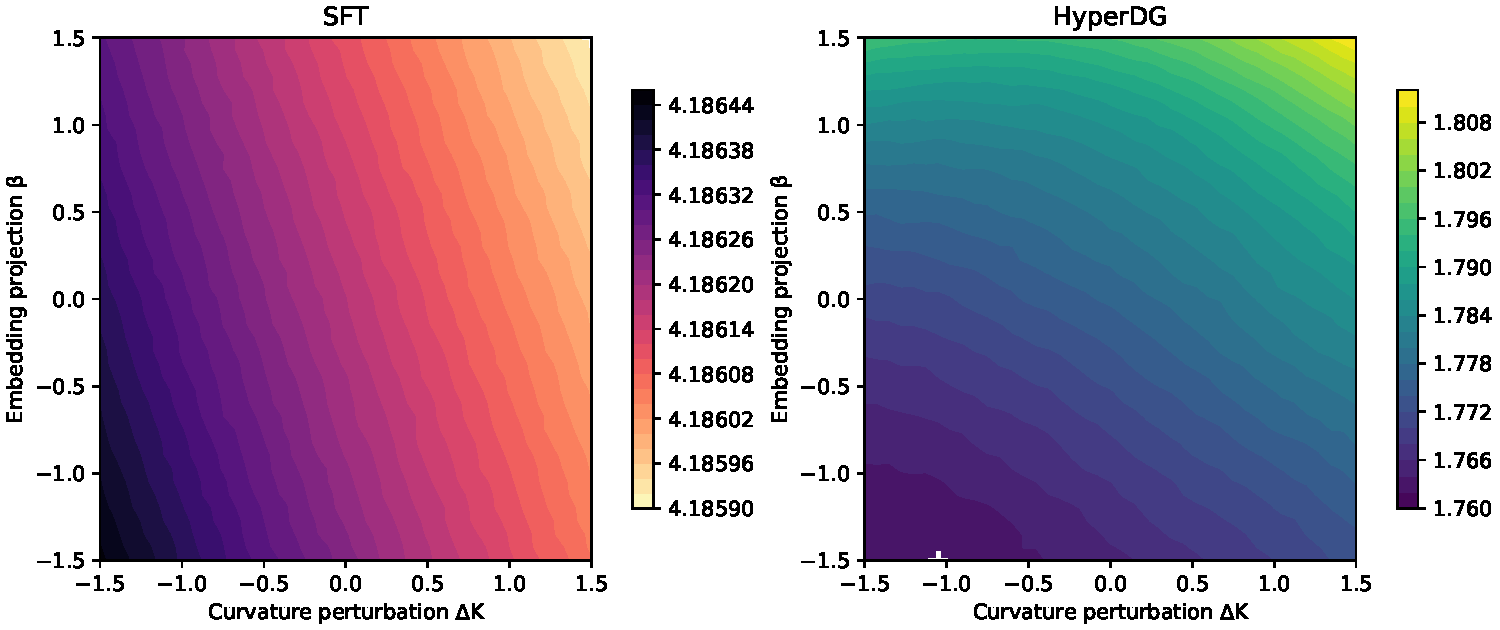
\includegraphics[width=\linewidth]{fig_loss_surface_officehome_split0.pdf}
        \caption{Office-Home}
    \end{subfigure}
    \hfill
    \begin{subfigure}[t]{0.32\linewidth}
        \centering
        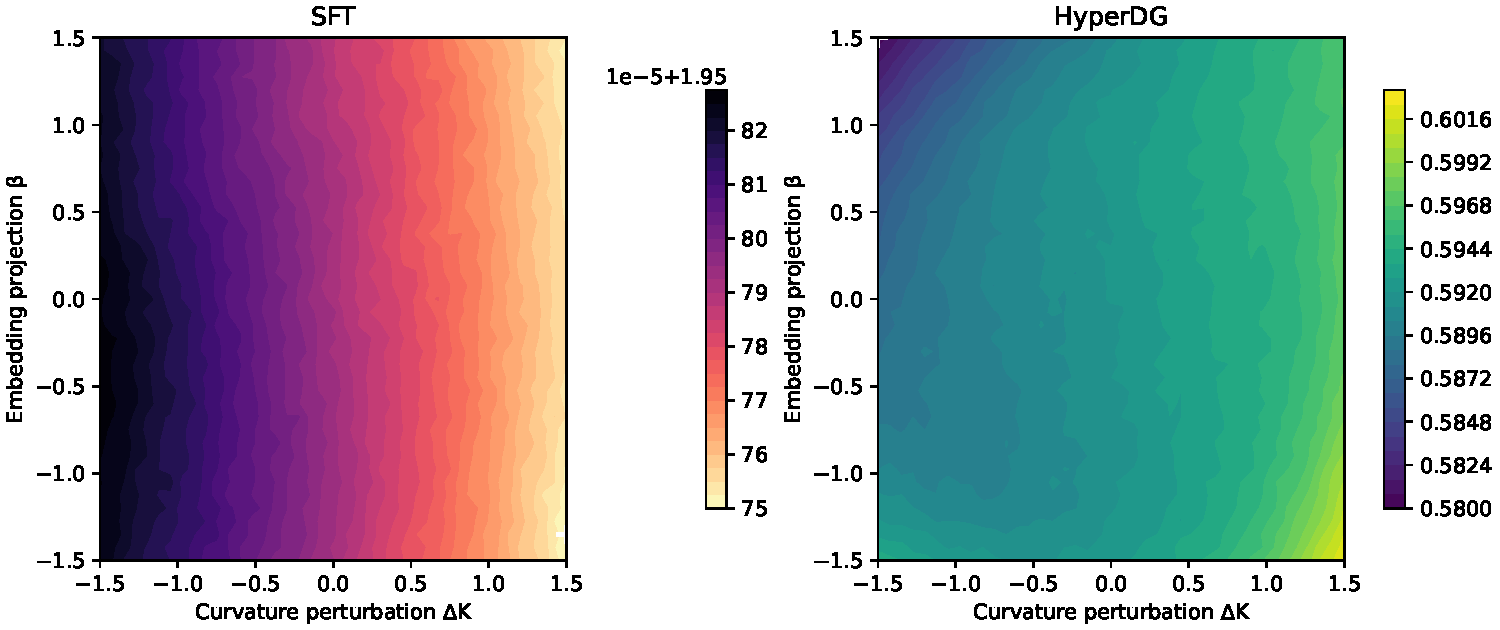
\includegraphics[width=\linewidth]{fig_loss_surface_pacs_split0.pdf}
        \caption{PACS}
    \end{subfigure}
    \hfill
    \begin{subfigure}[t]{0.32\linewidth}
        \centering
        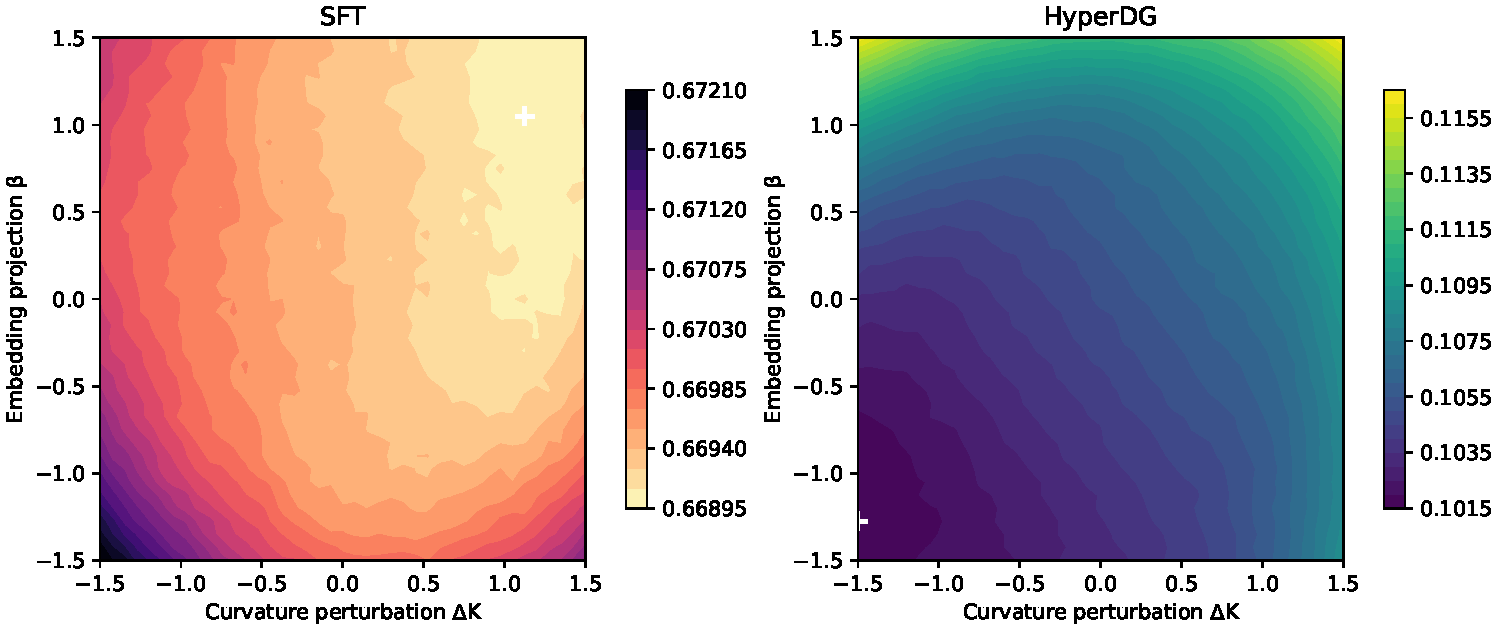
\includegraphics[width=\linewidth]{fig_loss_surface_vlcs_split0.pdf}
        \caption{VLCS}
    \end{subfigure}

    \caption{
    \textbf{Curvature response diagnostics across datasets.}
    For each domain, we perturb the curvature parameter $K$ within a fixed range 
    and measure the resulting change in embedding projection in hyperbolic space. 
    SFT (left of each plot) exhibits high sensitivity to curvature perturbations, 
    indicating unstable curvature--loss geometry and domain-dependent embedding 
    distortion. HyperDG (right) yields smoother, lower-magnitude responses, 
    reflecting reduced curvature divergence and improved geometric consistency.
    }
    \label{fig:curv_plots}
\end{figure}


Figure~\ref{fig:curv_plots} visualizes the stability of each domain's geometry
under small curvature perturbations. For baselines SFT that do not explicitly model curvature,
we evaluate curvature sensitivity by embedding their learned Euclidean features
into the same Lorentz manifold parameterized by curvature $K$ and perturbing $K$
at inference time. This ensures that curvature perturbations act as a common
geometric probe applied to the representation space, rather than relying on
method-specific curvature parameters.
For every domain, we slightly vary the
learned curvature $K_i$ within a fixed range around its final value and measure
how much the projected hyperbolic embeddings change. The horizontal axis shows
the curvature perturbation, while the vertical axis shows the resulting shift in
embedding projections.

SFT displays sharp and irregular responses, indicating that its geometry is
highly sensitive to small changes in curvature. HyperDG produces noticeably
flatter and smoother curves across all domains, reflecting more stable and
consistent geometry. This reduction in curvature sensitivity aligns with the
observed improvement in out-of-domain accuracy, confirming that HyperDG’s
generalization gains are closely tied to its curvature-stabilized
representations.




\section{Conclusion}

We present HyperDG, an iterative two-phase geometry-aware framework designed to mitigate manifold inconsistency arising from domain shifts. The method alternates between estimating a curvature-guided feedback signal that quantifies geometric misalignment across domains and refining per-domain curvature embeddings to enforce cross-domain consistency. By aligning domain geometries within a shared low-curvature basin, HyperDG achieves consistent and superior generalization over sharpness-aware and conventional DG methods on diverse benchmarks. This work highlights the value of geometric reasoning for improving model stability and transferability. Future efforts will focus on advancing theoretical analysis, developing efficient manifold parameterizations, and extending HyperDG toward multimodal and federated scenarios to promote scalable, geometry-driven generalization across heterogeneous learning settings.

\bibliography{main}
\bibliographystyle{tmlr}

\appendix
\section{Appendix}

% ===============================
\subsection{Theoretical Analysis and Intuition}
% ===============================

In Euclidean learning theory, generalization correlates with the
\emph{flatness} of minima in parameter space---models lying in wide
basins exhibit low sensitivity to perturbations and unseen data shifts.
In our Lorentzian formulation, curvature plays an analogous role but at
a higher geometric level: it defines the \emph{shape of the feature
manifold} rather than the shape of the loss basin. Ensuring
\emph{curvature consistency across domains} therefore extends
flat--minima robustness to manifold--level invariance.

\subsection{Riemannian Generalization Bound}
Let $\mathcal{M}_i=(\mathbb{L}^{d,1}_{K_i},g_{K_i})$ denote the
Lorentz manifold of domain~$i$ with curvature~$K_i$ and metric
tensor~$g_{K_i}$. For any hypothesis
$f:\mathcal{M}_i\!\to\!\mathcal{Y}$, the expected risk is
\begin{equation}
\mathcal{R}_{\mathcal{M}_i}(f)
   = \mathbb{E}_{(x,y)\sim P_i}\! \big[L(f(x),y)\big],
\end{equation}
and its empirical counterpart
$\hat{\mathcal{R}}_{\mathcal{M}_i}(f)$ is estimated from samples on
$\mathcal{M}_i$. Following the Riemannian PAC--Bayes analysis
\cite{liao2020pac}, the generalization gap satisfies
\begin{equation}
\big|\mathcal{R}_{\mathcal{M}_i}(f)
      - \hat{\mathcal{R}}_{\mathcal{M}_i}(f)\big|
\le
\mathcal{O}\!\left(
\sqrt{
\frac{\mathrm{KL}(Q\|P)
 + d_{\mathrm{Riem}}^2(\mathcal{M}_i,\mathcal{M}_s)}
      {n_i}}
\right),
\label{eq:riem_pac}
\end{equation}
where $d_{\mathrm{Riem}}$ is the Riemannian distance between the local
manifold~$\mathcal{M}_i$ and the shared tangent manifold~$\mathcal{M}_s$,
and $\mathrm{KL}(Q\|P)$ denotes the parameter--space divergence between
posterior~$Q$ and prior~$P$.

\subsection{Curvature Consistency as Distance Minimization}
The Lorentzian distance term in~\eqref{eq:riem_pac} depends on
curvature discrepancy:
\begin{equation}
d_{\mathrm{Riem}}^2(\mathcal{M}_i,\mathcal{M}_s)
  \propto
  \|K_i-K_s\|^2
  + \|\nabla g_{K_i}-\nabla g_{K_s}\|^2.
\label{eq:curv_dist}
\end{equation}
Minimizing curvature divergence ($L_{\text{curv}}$) directly
\emph{shrinks} this inter--manifold distance, tightening the
bound~\eqref{eq:riem_pac}. Hence, curvature alignment provably reduces
the variance term controlling generalization under domain shift.
Intuitively, when all domains share similar manifold geometry,
transporting features between them becomes nearly isometric and
preserves semantics.

\subsection{Analogy to Flat--Minima PAC--Bayes}
In Euclidean PAC Bayes theory
\cite{mcallester2003pac,lotfi2022pac},
flat minima correspond to parameter regions where the loss remains
stable under perturbations:
\begin{equation}
\mathcal{L}(\Theta+\epsilon)-\mathcal{L}(\Theta)\approx0,
\qquad
\forall\|\epsilon\|<\delta.
\end{equation}
Small Hessian eigenvalues imply broader flatness and tighter
generalization bounds.  Our Lorentzian extension replaces the Euclidean
Hessian curvature with the \emph{sectional curvature} of the feature
manifold:
\begin{equation}
\kappa(u,v)
=
\frac{
\langle R(u,v)v,u\rangle_{\mathbb{L}}
}{
\|u\|_{\mathbb{L}}^{2}\|v\|_{\mathbb{L}}^{2}
 - \langle u,v\rangle_{\mathbb{L}}^{2}
}.
\label{eq:sectional}
\end{equation}
Maintaining consistent $\kappa(u,v)$ across domains ensures that feature
perturbations along different manifold directions yield comparable
geodesic distortions, mirroring the flatness--in--loss--space condition.
Hence, \emph{flat--minima alignment}~$\Leftrightarrow$
\emph{curvature alignment} in the manifold domain.

\subsection{Bound for Multi-Domain Generalization}
Combining~\eqref{eq:riem_pac} and~\eqref{eq:curv_dist}, the cross--domain
generalization gap of the global model~$f_{\Theta_s}$ satisfies
\begin{equation}
\mathcal{E}_{\text{FDG}}
 =
\mathbb{E}_{i}\!
\big[
|\mathcal{R}_{\mathcal{M}_u}(f_{\Theta_s})
 -\mathcal{R}_{\mathcal{M}_i}(f_{\Theta_i})|
\big]
\le
\mathcal{O}\!\left(
\sqrt{
\frac{
\overline{\mathrm{KL}}
+\operatorname{Var}(K_i)}
{N}}
\right),
\label{eq:fdg_bound}
\end{equation}
where $\operatorname{Var}(K_i)$ measures curvature inconsistency among
domains. Minimizing $\operatorname{Var}(K_i)$ through the curvature
refinement step tightens the bound~\eqref{eq:fdg_bound}, guaranteeing
more stable cross--manifold transfer.

\subsection{Geometric Intuition}
\begin{enumerate}[label=(\alph*)]
  \item \textbf{Local Flatness $\to$ Global Curvature Consistency:}
        Flat minima ensure robustness to parameter perturbations,
        whereas curvature consistency ensures robustness to manifold
        perturbations---i.e., shifts in data geometry.
  \item \textbf{Tangent--Space Aggregation:}
        Aggregating in $T_o\mathbb{L}^{d,1}$ enforces local isometry
        among domains, reducing distortion in feature transport and
        stabilizing optimization trajectories.
  \item \textbf{Curvature Refinement Loop:}
        Iteratively updating $K_i$ drives domains toward a shared
        meta--manifold where gradients, Hessians, and curvatures
        co--align---the Lorentzian counterpart of refining toward a
        shared flat basin.
\end{enumerate}

\subsection{Theoretical Takeaway}
\begin{itemize}
  \item \textbf{Bound Tightening:}
        Minimizing curvature variance $\operatorname{Var}(K_i)$
        contracts the Riemannian generalization
        bound~\eqref{eq:fdg_bound}, yielding provably lower
        domain--shift sensitivity.
  \item \textbf{Unified Perspective:}
        Flat--minima consistency (Li \emph{et al.}, CVPR 2025)
        operates in Euclidean parameter space;
        FedGeoRefine extends this to Lorentzian feature space,
        achieving \emph{geometry--consistent generalization}.
  \item \textbf{Result:}
        A model trained with curvature refinement not only stabilizes
        local optimization but also learns a globally invariant geometry
        that generalizes naturally to unseen domains.
\end{itemize}

HyperDG formalizes the intuition that curvature alignment is the
manifold level analogue of flatness alignment.  By ensuring
curvature consistent manifolds across domains, it reduces geodesic
distortion under domain shift, yielding tighter theoretical and
empirical generalization.


\end{document}
